\documentclass[nobib]{tufte-handout}

\title{Exercise Session 1: Introduction -- what is graph theory? $\cdot$ 1MA020}

\author[Vilhelm Agdur]{Vilhelm Agdur\thanks{\href{mailto:vilhelm.agdur@math.uu.se}{\nolinkurl{vilhelm.agdur@math.uu.se}}}}

\date{23 October 2023}


%\geometry{showframe} % display margins for debugging page layout

\usepackage{graphicx} % allow embedded images
  \setkeys{Gin}{width=\linewidth,totalheight=\textheight,keepaspectratio}
  \graphicspath{{graphics/}} % set of paths to search for images
\usepackage{amsmath}  % extended mathematics
\usepackage{booktabs} % book-quality tables
\usepackage{units}    % non-stacked fractions and better unit spacing
\usepackage{multicol} % multiple column layout facilities
\usepackage{lipsum}   % filler text
\usepackage{fancyvrb} % extended verbatim environments
  \fvset{fontsize=\normalsize}% default font size for fancy-verbatim environments

\usepackage{color,soul} % Highlights for text

% Standardize command font styles and environments
\newcommand{\doccmd}[1]{\texttt{\textbackslash#1}}% command name -- adds backslash automatically
\newcommand{\docopt}[1]{\ensuremath{\langle}\textrm{\textit{#1}}\ensuremath{\rangle}}% optional command argument
\newcommand{\docarg}[1]{\textrm{\textit{#1}}}% (required) command argument
\newcommand{\docenv}[1]{\textsf{#1}}% environment name
\newcommand{\docpkg}[1]{\texttt{#1}}% package name
\newcommand{\doccls}[1]{\texttt{#1}}% document class name
\newcommand{\docclsopt}[1]{\texttt{#1}}% document class option name
\newenvironment{docspec}{\begin{quote}\noindent}{\end{quote}}% command specification environment

\include{mathcommands.extratex}

\begin{document}

\maketitle% this prints the handout title, author, and date

\begin{abstract}
\noindent
We begin the course by motivating in general what graph theory is, and the different kinds of thing it can be used to study. We also use these examples in our exercises to start to build up our graph-theoretical vocabulary.
\end{abstract}

What is graph theory? It is, unsurprisingly, the study of graphs. Not graphs as in ``we plot the function $x^2+3x+2$'', but graphs as in things that look like this:

\begin{figure}
  \centering
  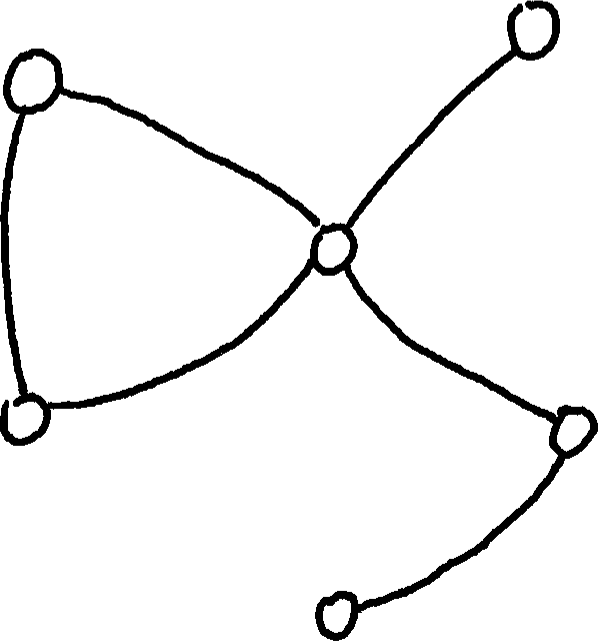
\includegraphics[width=0.3\textwidth]{graphics/L1_exc/unlabeled_simple_graph.png}
  \caption{A simple graph.}
  \label{fig:simple_graph}
\end{figure}

A graph consists, as indicated in Figure \ref{fig:simple_graph}, of \emph{vertices} connected by \emph{edges}. This is the most basic situation we can have, where there are finitely many vertices and each pair of vertices either have an edge between them or not. We will fairly regularly be considering various extensions of this notion, to contain more information. For example, we can add labels to the vertices,\sidenote[][-1cm]{In fact, we will see when we get to the formal definitions that this is probably the most basic notion -- the unlabelled version turns out to be subtler to define.} as in Figure \ref{fig:labelled_simple_graph}.

\begin{figure}
  \centering
  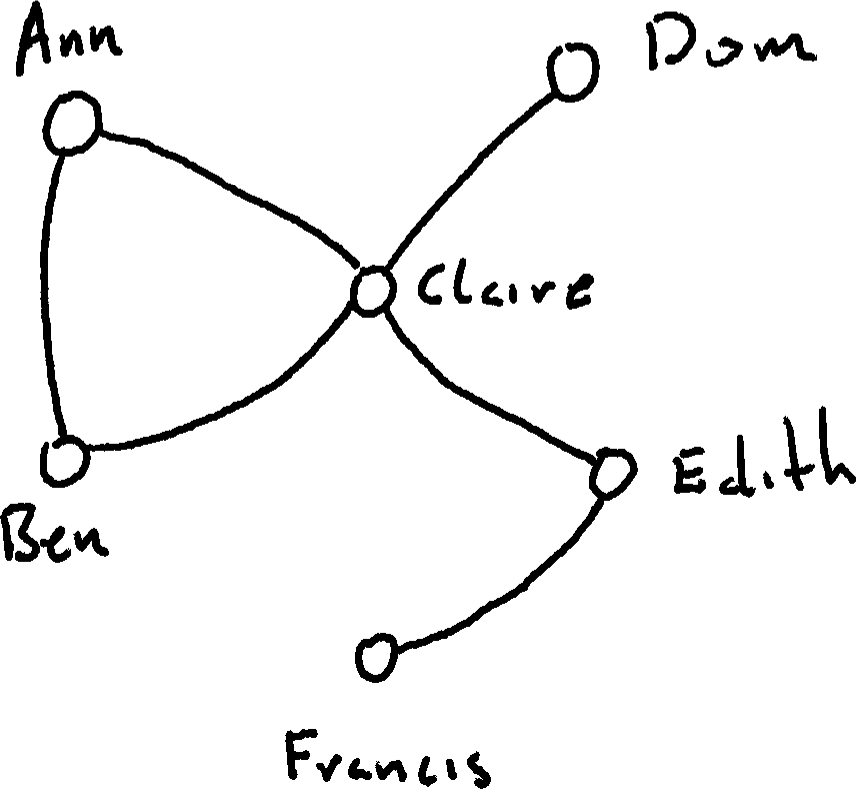
\includegraphics[width=0.3\textwidth]{graphics/L1_exc/labeled_simple_graph.png}
  \caption{A labelled simple graph.}
  \label{fig:labelled_simple_graph}
\end{figure}

The labels we added also start to make clear what kind of real-world thing a graph might model -- if we interpret an edge as saying ``these people are friends'', we have a tiny example of a social network represented as a graph.\sidenote[][]{Now imagine in your head what it would look like if vertices were Facebook accounts and edges were ``are friends'' -- a much larger graph, but an example of the same thing. What might be interesting questions to ask about this graph?

This interpretation of vertices as people and edges as friendships will be common throughout the course, because it is natural given my research interests, and it is an easy down-to-earth example.}

It's not only the vertices we can write things on -- often it is interesting to give each edge a number, called its \emph{weight}, like in Figure \ref{fig:weighted_graph}. Maybe the numbers represent how many hours per day they spend together.

\begin{figure}
  \centering
  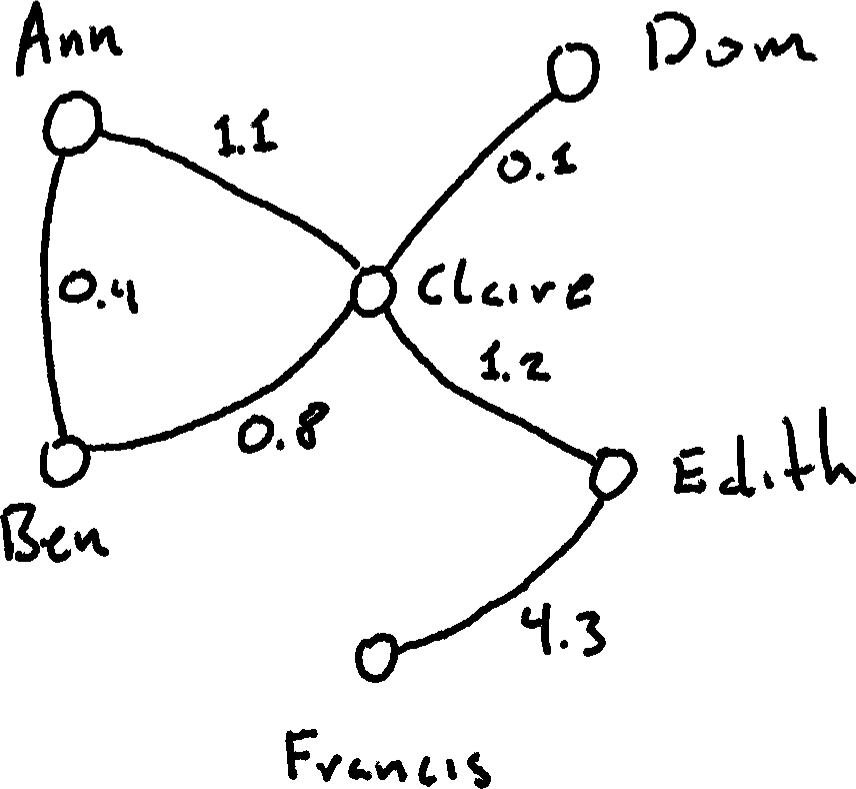
\includegraphics[width=0.3\textwidth]{graphics/L1_exc/weighted_graph.png}
  \caption{A weighted graph.}
  \label{fig:weighted_graph}
\end{figure}

Another common version is to permit multiple edges between vertices, as in Figure \ref{fig:labelled_multigraph}. Perhaps each edge represents a class the two people have in common, so it makes sense to have more than one edge?\sidenote[][-1.5cm]{If you think about it, this is similar to just labelling a single edge with an integer saying how many classes they have in common. However, it has a very different feeling, and the maths we do on multigraphs will be quite different from what we do on weighted graphs.}

\begin{figure}
  \centering
  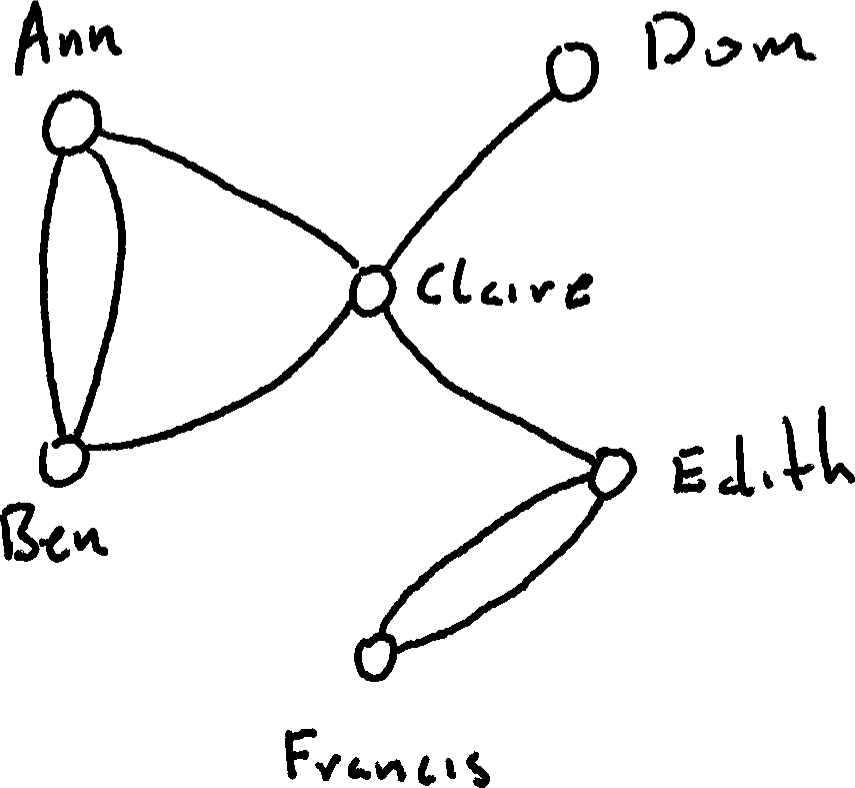
\includegraphics[width=0.3\textwidth]{graphics/L1_exc/multigraph.png}
  \caption[][1cm]{A labelled multigraph.}
  \label{fig:labelled_multigraph}
\end{figure}

Or perhaps the edges have a direction, as in Figure \ref{fig:labelled_digraph}? Now the interpretation might be that an edge means ``is in love with''.\sidenote[][-0.5cm]{So in our figure there is quite a bit of unrequited love and confused emotions -- though perhaps Edith and Francis will find happiness?}

\begin{figure}
  \centering
  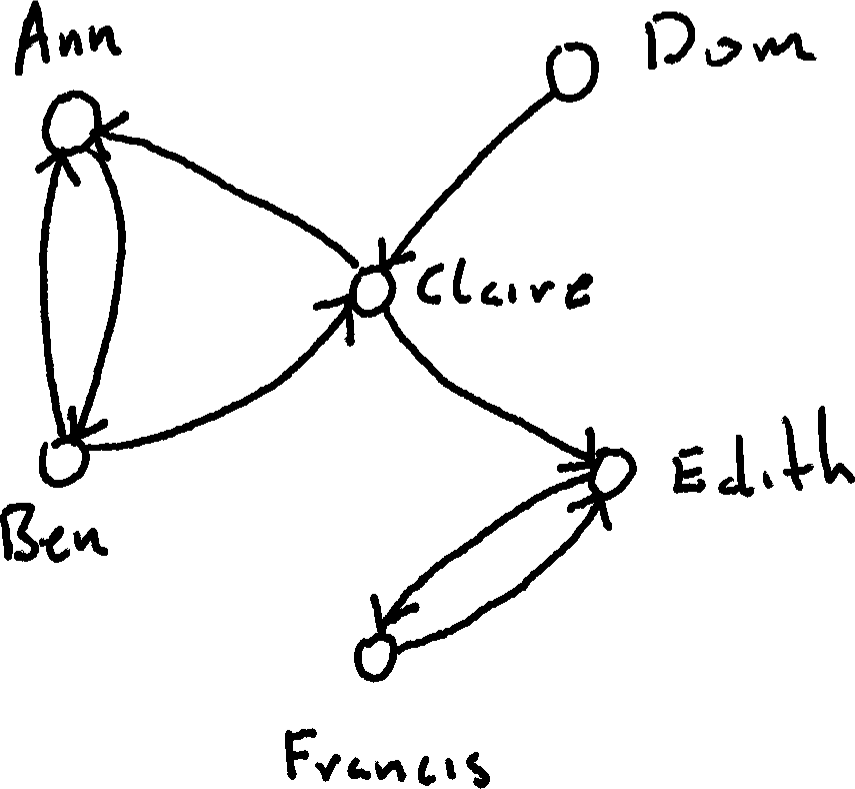
\includegraphics[width=0.3\textwidth]{graphics/L1_exc/digraph.png}
  \caption[][0.8cm]{A directed graph.}
  \label{fig:labelled_digraph}
\end{figure}

The final version that we will actually see used in the course is to give the vertices (or the edges) colours, as in Figure \ref{fig:vertex_coloured_graph}. Now the colour might represent the gender of a person, or some other classification of vertices into various types.

\begin{figure}
  \centering
  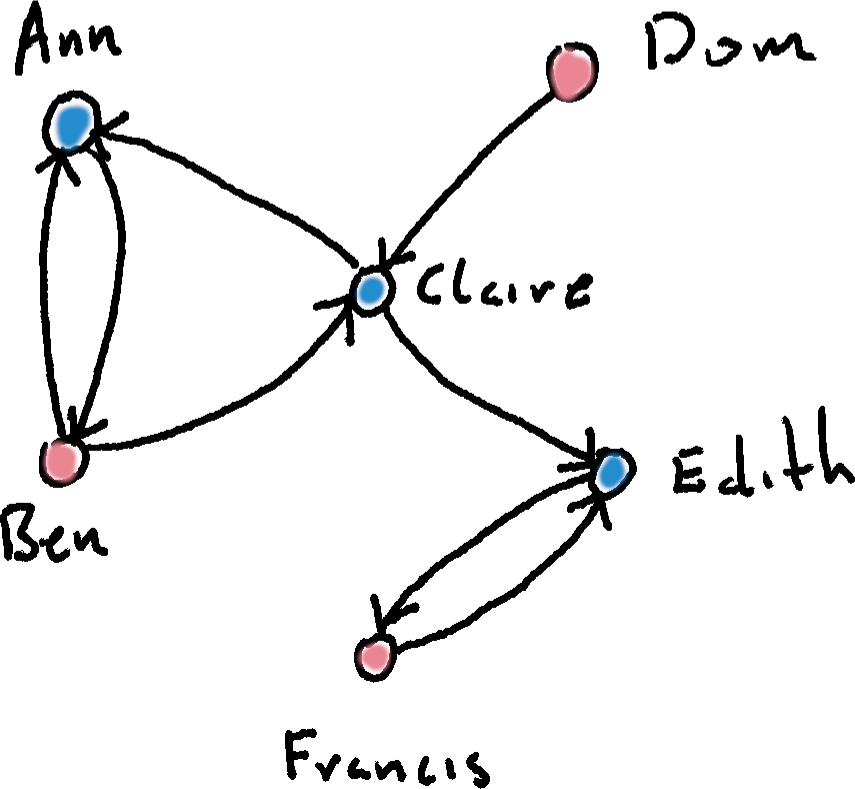
\includegraphics[width=0.3\textwidth]{graphics/L1_exc/vertex_coloured_digraph.png}
  \caption{A directed graph with a vertex colouring.}
  \label{fig:vertex_coloured_graph}
\end{figure}

As we proceed in the course, we will of course give precise mathematical definitions of what exactly each of these types of graph is. For today, however, we don't really need those definitions -- the intuitive descriptions will be enough.

\section{Exercise topic 1: Euler in Königsberg}

The very first thing studied in graph theory, in the early eighteenth century, was the bridges of Königsberg. Königsberg -- today Kaliningrad -- is divided into four parts by the river Pregel, and at the time the city had seven bridges, as in Figure \ref{fig:konigsberg_map}.

\begin{figure}
  \centering
  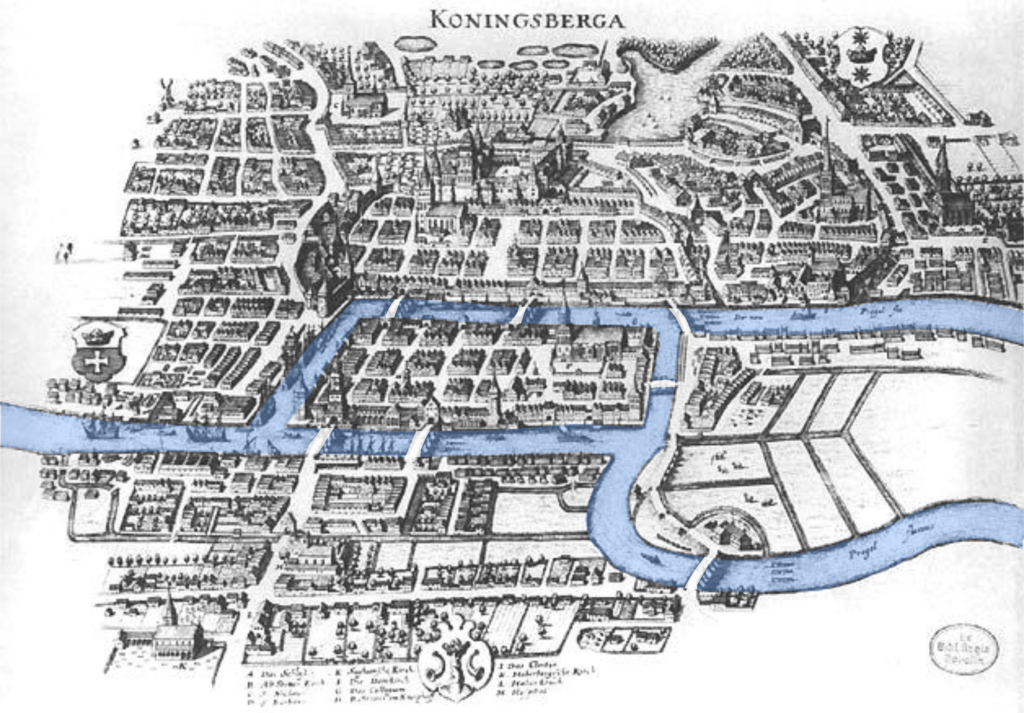
\includegraphics[width=0.9\textwidth]{graphics/L1_exc/konigsberg_map.png}
  \caption{A map of the city of Königsberg.}
  \label{fig:konigsberg_map}
\end{figure}

\begin{xca}
  Can you represent this situation as a graph? Which of the six types of graph we looked at earlier would be most appropriate?
\end{xca}

One question the people of this town would ask themselves, for some reason,\sidenote[][]{Presumably they were all very bored all the time, since they didn't have TikTok yet to keep themselves distracted.} was the following: Is it possible to take a walk around town that uses each bridge exactly once, and takes you back to where you started?

\begin{xca}
  Is it? Convince yourselves that it is not by trying to find such a walk. Can you make it possible by adding or removing edges?

  Try to draw some other graphs where it is possible, and ones where it is not -- can you find some pattern? There is a simple rule to when it is possible or not -- can you figure out what it might be?
\end{xca}

The person who originally solved this problem was the great Leonhard Euler -- in the lecture tomorrow we will see a proof of his result.

If you want to continue on with this exercise and try to prove that the pattern you found always holds, do try and please ask for hints if you need one. It might be rather difficult for you to find the right technique, but it could be a productive sort of difficulty. Or move on to the next exercise.

\section{Exercise topic 2: Same same, but different}

\begin{xca}
    \hl{a figure of two isomorphic graphs with different labels -- exercise: ``figure out a way to describe why these are really the same''}
\end{xca}

%\bibliography{references}
%\bibliographystyle{plainnat}

\end{document}
